\documentclass[a4paper]{article}

\author{Camil Staps}
\title{Fuspel}
\date{\gitcommitdate[formatDate]}

\usepackage[T1]{fontenc}
\usepackage{lmodern}
\usepackage[scaled]{beramono}

\usepackage{geometry}
\usepackage[usenames,dvipsnames,svgnames,table]{xcolor}
\definecolor{linkcolor}{rgb}{0.65,0,0}
\definecolor{citecolor}{rgb}{0,0.65,0}
\definecolor{urlcolor}{rgb}{0,0,0.65}
\usepackage[
    colorlinks=true,
    linkcolor=linkcolor,
    urlcolor=urlcolor,
    citecolor=citecolor]{hyperref}

\usepackage{latexgit}

\usepackage{tikz}

\usepackage{syntax}
\usepackage{fuspel}

\lstset{
	basicstyle=\small\ttfamily,
	keywordstyle=\bfseries,
	language=fuspel
}

\begin{document}

\maketitle

\begin{abstract}
	This document describes Fuspel,
	a minimal, untyped, lazy functional programming language
	based on term graph rewriting.
	It can run with even a few kB of RAM.
	This document describes the language's syntax and semantics.
	It accompanies version \gitcommithash{} of the C interpreter at
	\url{https://github.com/camilstaps/fuspel}, committed at
	\gitcommitdate[formatDate,formatTime].
\end{abstract}

\tableofcontents

\section{Examples}
\label{sec:examples}

\subsection{A basic example}
\label{sec:examples:basic}

\begin{lstlisting}
	id x      = x;
	const x y = x;
	fst (a,_) = a;
	double x  = (x, x);
	main      = fst (const (double 5) (double 10));
\end{lstlisting}

The program is rewritten as in \autoref{fig:rewrite:examples:basic}.

\begin{figure}[h]
	\centering
	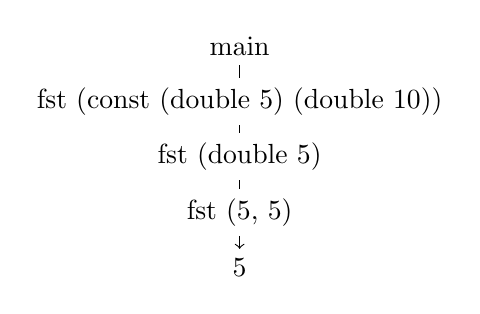
\begin{tikzpicture}[->,node distance=2em]
		\node              (r0) {\fuspel{main}};
		\node[below of=r0] (r1) {\fuspel{fst (const (double 5) (double 10))}};
		\node[below of=r1] (r2) {\fuspel{fst (double 5)}};
		\node[below of=r2] (r3) {\fuspel{fst (5, 5)}};
		\node[below of=r3] (r4) {\fuspel{5}};
		\path[draw] (r0) -- (r1) -- (r2) -- (r3) -- (r4);
	\end{tikzpicture}
	\caption{Basic rewriting example.\label{fig:rewrite:examples:basic}}
\end{figure}

\subsection{The code keyword}
\label{sec:examples:code}

With the \fuspel{code} keyword it is possible to link to C code. This works as
follows:

\begin{lstlisting}
	mul a b = code mul a b;
	sub a b = code sub a b;
	fac 1   = 1;
	fac n   = mul n (fac (sub 1 n));
	main    = fac 3;
\end{lstlisting}

To rewrite a \fuspel{code} expression, all its arguments have to be evaluated
completely. The corresponding C function is looked up and executed on its
arguments. The expression is rewritten with the result of the function call.

The code name \fuspel{mul} stands for integer multiplication, \fuspel{sub} for
subtraction. Hence, the example is rewritten as:

\begin{lstlisting}
	main
	     fac 3
	     mul 3 (     fac (     sub 1 3)        )
	     mul 3 (     fac (code sub 1 3)        )
	     mul 3 (     fac 2                     )
	     mul 3 (     mul 2 (fac (     sub 1 2)))
	     mul 3 (     mul 2 (fac (code sub 1 2)))
	     mul 3 (     mul 2 (fac 1)             )
	     mul 3 (     mul 2 1                   )
	     mul 3 (code mul 2 1                   )
	     mul 3 2
	code mul 3 2
	6
\end{lstlisting}

A complete overview of the \fuspel{code} names can be found in
\autoref{sec:code}.

\subsection{Strictness}
\label{sec:examples:strictness}

By default, expressions are rewritten using the leftmost outermost rewriting
strategy. This is guaranteed to find a normal form if one exists, but can be
inefficient as it can lead to duplicate calculation. Consider the following
example:

\begin{lstlisting}
	mul x y  = code mul x y;
	double x = (x, x);
	main     = double (mul 5 10);
\end{lstlisting}

The result is \fuspel{(50,50)}. The expression is rewritten to \fuspel{(mul 5
10, mul 5 10)}, and only then the \fuspel{mul} calls are rewritten. This is
inefficient, because we have to multiply the numbers twice.

We can force another rewriting strategy by adding a strictness annotation
(\fuspel{!}) to the argument of \fuspel{double}:

\begin{lstlisting}
	mul x y   = code mul x y;
	double !x = (x, x);
	main      = double (mul 5 10);
\end{lstlisting}

The result is the same, but the multiplication is only executed once. To apply
the \fuspel{double} rule, its argument must be fully evaluated due to the
strictness annotation. Therefore, the expression is first rewritten to
\fuspel{double 50}.

One must be careful with adding strictness annotations. Consider the following
program:

\begin{lstlisting}
	mul x y     = code mul x y;
	app f (a,b) = (f a, f b);
	fst (x,_)   = x;
	double !x   = (x, x);
	main        = app fst (double (mul 5 10, mul 10 20));
\end{lstlisting}

In the call to \fuspel{double}, both \fuspel{mul 5 10} and \fuspel{mul 10 20}
are fully rewritten due to the strictness annotation. However, only the first
elements of the resulting tuples are used: the result is \fuspel{(50,50)}. We
did not need to fully rewrite \fuspel{mul 10 20}, so the strictness annotation
gave us more work.


\appendix

\clearpage
\section{Grammar}
\label{sec:grammar}

\setlength{\grammarparsep}{4pt}
\setlength{\grammarindent}{10em}
\begin{grammar}
	<Fuspel> ::= <Rewrite-list>

	<Rewrite-list> ::= <Rewrite> `;' <Rewrite-list> | <empty>

	<Rewrite> ::= <Name> <Arg-list> `=' <Rhs>

	<Arg-list> ::= <Arg> ` ' <Arg-list> | <empty>

	<Arg> ::= <Simple-expr>

	<Simple-expr> ::= <Int>
		\alt <Name>
		\alt <Simple-list>
		\alt <Simple-tuple>

	<Simple-list> ::= `[' <Simple-expr> `:' <Simple-list> `]'
		\alt `[]'
	
	<Simple-tuple> ::= `(' <Simple-expr> `,' <Simple-expr> `)'

	<Rhs> ::= <Expr>

	<Expr> ::= <Int>
		\alt <Name>
		\alt <List>
		\alt <Tuple>
		\alt <Expr> <Expr>
		\alt `code' <Name>
		\alt `(' <Expr> `)'

	<List> ::= `[' <Expr> `:' <List> `]'
		\alt `[]'
	
	<Tuple> ::= `(' <Simple-expr> `,' <Simple-expr> `)'
\end{grammar}

\clearpage
\section{Builtin code names}
\label{sec:code}


\begin{center}
{\renewcommand{\arraystretch}{1.3}
	\begin{tabular}{l l l}
		\textbf{Name} & \textbf{Type} & \textbf{Description} \\

		\hline\hline\multicolumn{3}{l}{\emph{Integer operations}} \\\hline
		\fuspel{add a b}
			& Int $\to$ Int $\to$ Int
			& Adds $a$ and $b$ \\
		\fuspel{mul a b}
			& Int $\to$ Int $\to$ Int
			& Multiplies $a$ and $b$ \\
		\fuspel{sub a b}
			& Int $\to$ Int $\to$ Int
			& Subtracts $a$ from $b$ \\

		\hline \multicolumn{3}{l}{\emph{Tests}} \\\hline
		\fuspel{eq a b}
			& Int $\to$ Int $\to \{0,1\}$
			& 1 if $a=b$, 0 otherwise \\
		\fuspel{ge a b}
			& Int $\to$ Int $\to \{0,1\}$
			& 1 if $a\ge b$, 0 otherwise \\
		\fuspel{gt a b}
			& Int $\to$ Int $\to \{0,1\}$
			& 1 if $a>b$, 0 otherwise \\
		\fuspel{le a b}
			& Int $\to$ Int $\to \{0,1\}$
			& 1 if $a\le b$, 0 otherwise \\
		\fuspel{lt a b}
			& Int $\to$ Int $\to \{0,1\}$
			& 1 if $a<b$, 0 otherwise \\
		\fuspel{ne a b}
			& Int $\to$ Int $\to \{0,1\}$
			& 1 if $a\neq b$, 0 otherwise \\

		\hline\multicolumn{3}{l}{\emph{Miscellaneous}} \\\hline
		\fuspel{time}
			& Int
			& The current time in seconds since the Unix Epoch. \\
	\end{tabular}
}
\end{center}


\end{document}
